\documentclass[1p]{elsarticle_modified}
%\bibliographystyle{elsarticle-num}

%\usepackage[colorlinks]{hyperref}
%\usepackage{abbrmath_seonhwa} %\Abb, \Ascr, \Acal ,\Abf, \Afrak
\usepackage{amsfonts}
\usepackage{amssymb}
\usepackage{amsmath}
\usepackage{amsthm}
\usepackage{scalefnt}
\usepackage{amsbsy}
\usepackage{kotex}
\usepackage{caption}
\usepackage{subfig}
\usepackage{color}
\usepackage{graphicx}
\usepackage{xcolor} %% white, black, red, green, blue, cyan, magenta, yellow
\usepackage{float}
\usepackage{setspace}
\usepackage{hyperref}

\usepackage{tikz}
\usetikzlibrary{arrows}

\usepackage{multirow}
\usepackage{array} % fixed length table
\usepackage{hhline}

%%%%%%%%%%%%%%%%%%%%%
\makeatletter
\renewcommand*\env@matrix[1][\arraystretch]{%
	\edef\arraystretch{#1}%
	\hskip -\arraycolsep
	\let\@ifnextchar\new@ifnextchar
	\array{*\c@MaxMatrixCols c}}
\makeatother %https://tex.stackexchange.com/questions/14071/how-can-i-increase-the-line-spacing-in-a-matrix
%%%%%%%%%%%%%%%

\usepackage[normalem]{ulem}

\newcommand{\msout}[1]{\ifmmode\text{\sout{\ensuremath{#1}}}\else\sout{#1}\fi}
%SOURCE: \msout is \stkout macro in https://tex.stackexchange.com/questions/20609/strikeout-in-math-mode

\newcommand{\cancel}[1]{
	\ifmmode
	{\color{red}\msout{#1}}
	\else
	{\color{red}\sout{#1}}
	\fi
}

\newcommand{\add}[1]{
	{\color{blue}\uwave{#1}}
}

\newcommand{\replace}[2]{
	\ifmmode
	{\color{red}\msout{#1}}{\color{blue}\uwave{#2}}
	\else
	{\color{red}\sout{#1}}{\color{blue}\uwave{#2}}
	\fi
}

\newcommand{\Sol}{\mathcal{S}} %segment
\newcommand{\D}{D} %diagram
\newcommand{\A}{\mathcal{A}} %arc


%%%%%%%%%%%%%%%%%%%%%%%%%%%%%5 test

\def\sl{\operatorname{\textup{SL}}(2,\Cbb)}
\def\psl{\operatorname{\textup{PSL}}(2,\Cbb)}
\def\quan{\mkern 1mu \triangleright \mkern 1mu}

\theoremstyle{definition}
\newtheorem{thm}{Theorem}[section]
\newtheorem{prop}[thm]{Proposition}
\newtheorem{lem}[thm]{Lemma}
\newtheorem{ques}[thm]{Question}
\newtheorem{cor}[thm]{Corollary}
\newtheorem{defn}[thm]{Definition}
\newtheorem{exam}[thm]{Example}
\newtheorem{rmk}[thm]{Remark}
\newtheorem{alg}[thm]{Algorithm}

\newcommand{\I}{\sqrt{-1}}
\begin{document}

%\begin{frontmatter}
%
%\title{Boundary parabolic representations of knots up to 8 crossings}
%
%%% Group authors per affiliation:
%\author{Yunhi Cho} 
%\address{Department of Mathematics, University of Seoul, Seoul, Korea}
%\ead{yhcho@uos.ac.kr}
%
%
%\author{Seonhwa Kim} %\fnref{s_kim}}
%\address{Center for Geometry and Physics, Institute for Basic Science, Pohang, 37673, Korea}
%\ead{ryeona17@ibs.re.kr}
%
%\author{Hyuk Kim}
%\address{Department of Mathematical Sciences, Seoul National University, Seoul 08826, Korea}
%\ead{hyukkim@snu.ac.kr}
%
%\author{Seokbeom Yoon}
%\address{Department of Mathematical Sciences, Seoul National University, Seoul, 08826,  Korea}
%\ead{sbyoon15@snu.ac.kr}
%
%\begin{abstract}
%We find all boundary parabolic representation of knots up to 8 crossings.
%
%\end{abstract}
%\begin{keyword}
%    \MSC[2010] 57M25 
%\end{keyword}
%
%\end{frontmatter}

%\linenumbers
%\tableofcontents
%
\newcommand\colored[1]{\textcolor{white}{\rule[-0.35ex]{0.8em}{1.4ex}}\kern-0.8em\color{red} #1}%
%\newcommand\colored[1]{\textcolor{white}{ #1}\kern-2.17ex	\textcolor{white}{ #1}\kern-1.81ex	\textcolor{white}{ #1}\kern-2.15ex\color{red}#1	}

{\Large $\underline{12n_{0508}~(K12n_{0508})}$}

\setlength{\tabcolsep}{10pt}
\renewcommand{\arraystretch}{1.6}
\vspace{1cm}\begin{tabular}{m{100pt}>{\centering\arraybackslash}m{274pt}}
\multirow{5}{120pt}{
	\centering
	\includegraphics[width=112pt]{../../../GIT/diagram.site/Diagrams/png/2597_12n_0508.png}\\
\ \ \ A knot diagram\footnotemark}&
\allowdisplaybreaks
\textbf{Linearized knot diagam} \\
\cline{2-2}
 &
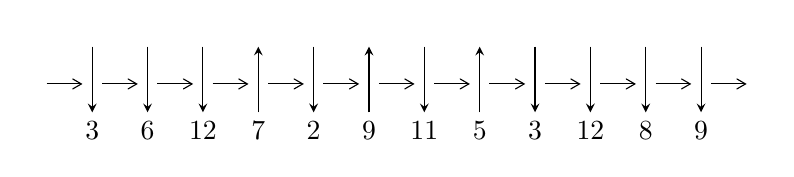
\begin{tikzpicture}[x=20pt, y=17pt]
	% nodes
	\node (C0) at (0, 0) {};
	\node (C1) at (1, 0) {};
	\node (C1U) at (1, +1) {};
	\node (C1D) at (1, -1) {3};

	\node (C2) at (2, 0) {};
	\node (C2U) at (2, +1) {};
	\node (C2D) at (2, -1) {6};

	\node (C3) at (3, 0) {};
	\node (C3U) at (3, +1) {};
	\node (C3D) at (3, -1) {12};

	\node (C4) at (4, 0) {};
	\node (C4U) at (4, +1) {};
	\node (C4D) at (4, -1) {7};

	\node (C5) at (5, 0) {};
	\node (C5U) at (5, +1) {};
	\node (C5D) at (5, -1) {2};

	\node (C6) at (6, 0) {};
	\node (C6U) at (6, +1) {};
	\node (C6D) at (6, -1) {9};

	\node (C7) at (7, 0) {};
	\node (C7U) at (7, +1) {};
	\node (C7D) at (7, -1) {11};

	\node (C8) at (8, 0) {};
	\node (C8U) at (8, +1) {};
	\node (C8D) at (8, -1) {5};

	\node (C9) at (9, 0) {};
	\node (C9U) at (9, +1) {};
	\node (C9D) at (9, -1) {3};

	\node (C10) at (10, 0) {};
	\node (C10U) at (10, +1) {};
	\node (C10D) at (10, -1) {12};

	\node (C11) at (11, 0) {};
	\node (C11U) at (11, +1) {};
	\node (C11D) at (11, -1) {8};

	\node (C12) at (12, 0) {};
	\node (C12U) at (12, +1) {};
	\node (C12D) at (12, -1) {9};
	\node (C13) at (13, 0) {};

	% arrows
	\draw[->,>={angle 60}]
	(C0) edge (C1) (C1) edge (C2) (C2) edge (C3) (C3) edge (C4) (C4) edge (C5) (C5) edge (C6) (C6) edge (C7) (C7) edge (C8) (C8) edge (C9) (C9) edge (C10) (C10) edge (C11) (C11) edge (C12) (C12) edge (C13) ;	\draw[->,>=stealth]
	(C1U) edge (C1D) (C2U) edge (C2D) (C3U) edge (C3D) (C4D) edge (C4U) (C5U) edge (C5D) (C6D) edge (C6U) (C7U) edge (C7D) (C8D) edge (C8U) (C9U) edge (C9D) (C10U) edge (C10D) (C11U) edge (C11D) (C12U) edge (C12D) ;
	\end{tikzpicture} \\
\hhline{~~} \\& 
\textbf{Solving Sequence} \\ \cline{2-2} 
 &
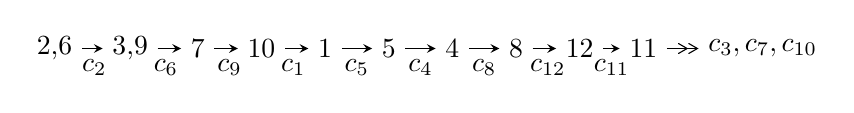
\begin{tikzpicture}[x=23pt, y=7pt]
	% node
	\node (A0) at (-1/8, 0) {2,6};
	\node (A1) at (17/16, 0) {3,9};
	\node (A2) at (17/8, 0) {7};
	\node (A3) at (25/8, 0) {10};
	\node (A4) at (33/8, 0) {1};
	\node (A5) at (41/8, 0) {5};
	\node (A6) at (49/8, 0) {4};
	\node (A7) at (57/8, 0) {8};
	\node (A8) at (65/8, 0) {12};
	\node (A9) at (73/8, 0) {11};
	\node (C1) at (1/2, -1) {$c_{2}$};
	\node (C2) at (13/8, -1) {$c_{6}$};
	\node (C3) at (21/8, -1) {$c_{9}$};
	\node (C4) at (29/8, -1) {$c_{1}$};
	\node (C5) at (37/8, -1) {$c_{5}$};
	\node (C6) at (45/8, -1) {$c_{4}$};
	\node (C7) at (53/8, -1) {$c_{8}$};
	\node (C8) at (61/8, -1) {$c_{12}$};
	\node (C9) at (69/8, -1) {$c_{11}$};
	\node (A10) at (11, 0) {$c_{3},c_{7},c_{10}$};

	% edge
	\draw[->,>=stealth]	
	(A0) edge (A1) (A1) edge (A2) (A2) edge (A3) (A3) edge (A4) (A4) edge (A5) (A5) edge (A6) (A6) edge (A7) (A7) edge (A8) (A8) edge (A9) ;
	\draw[->>,>={angle 60}]	
	(A9) edge (A10);
\end{tikzpicture} \\ 

\end{tabular} \\

\footnotetext{
The image of knot diagram is generated by the software ``\textbf{Draw programme}" developed by Andrew Bartholomew(\url{http://www.layer8.co.uk/maths/draw/index.htm\#Running-draw}), where we modified some parts for our purpose(\url{https://github.com/CATsTAILs/LinksPainter}).
}\phantom \\ \newline 
\centering \textbf{Ideals for irreducible components\footnotemark of $X_{\text{par}}$} 
 
\begin{align*}
I^u_{1}&=\langle 
-11 u^{14}+3 u^{13}+\cdots+36 b+14,\;- u^{14}+3 u^{13}+\cdots+12 a-8,\\
\phantom{I^u_{1}}&\phantom{= \langle  }u^{15}+2 u^{14}-2 u^{13}-5 u^{12}+4 u^{11}+9 u^{10}+u^9+u^8+3 u^7-4 u^6+5 u^5+21 u^4+16 u^3+4 u^2-2\rangle \\
I^u_{2}&=\langle 
-7 u^{24}+2 u^{23}+\cdots+32 b+140,\;-47 u^{25}-117 u^{24}+\cdots+368 a+2737,\;u^{26}+2 u^{25}+\cdots-46 u-23\rangle \\
I^u_{3}&=\langle 
u^3- u^2+2 b,\;- u^2+2 a+u,\;u^4- u^2+2\rangle \\
I^u_{4}&=\langle 
4 b^2-4 b-32 u+33,\;2 b u-2 b- u+1,\;2 a+1,\;u^2-2 u+1\rangle \\
I^u_{5}&=\langle 
- u^3+u^2+2 b- u+1,\;u^3+u^2+2 a- u+1,\;u^4+1\rangle \\
I^u_{6}&=\langle 
- a^2+b-2 a,\;a^3+2 a^2+a+1,\;u-1\rangle \\
I^u_{7}&=\langle 
b a- a^2+a+1,\;u-1\rangle \\
I^u_{8}&=\langle 
b- a-1,\;u-1\rangle \\
\\
I^v_{1}&=\langle 
a,\;b^3- b-1,\;v-1\rangle \\
I^v_{2}&=\langle 
a,\;b+1,\;v-1\rangle \\
\end{align*}
\raggedright * 8 irreducible components of $\dim_{\mathbb{C}}=0$, with total 59 representations.\\
\raggedright * 2 irreducible components of $\dim_{\mathbb{C}}=1$ \\
\footnotetext{All coefficients of polynomials are rational numbers. But the coefficients are sometimes approximated in decimal forms when there is not enough margin.}
\newpage
\renewcommand{\arraystretch}{1}
\centering \section*{I. $I^u_{1}= \langle -11 u^{14}+3 u^{13}+\cdots+36 b+14,\;- u^{14}+3 u^{13}+\cdots+12 a-8,\;u^{15}+2 u^{14}+\cdots+4 u^2-2 \rangle$}
\flushleft \textbf{(i) Arc colorings}\\
\begin{tabular}{m{7pt} m{180pt} m{7pt} m{180pt} }
\flushright $a_{2}=$&$\begin{pmatrix}1\\0\end{pmatrix}$ \\
\flushright $a_{6}=$&$\begin{pmatrix}0\\u\end{pmatrix}$ \\
\flushright $a_{3}=$&$\begin{pmatrix}1\\u^2\end{pmatrix}$ \\
\flushright $a_{9}=$&$\begin{pmatrix}\frac{1}{12} u^{14}-\frac{1}{4} u^{13}+\cdots+\frac{1}{6} u+\frac{2}{3}\\\frac{11}{36} u^{14}-\frac{1}{12} u^{13}+\cdots-\frac{8}{9} u-\frac{7}{18}\end{pmatrix}$ \\
\flushright $a_{7}=$&$\begin{pmatrix}\frac{1}{4} u^{12}-\frac{3}{4} u^{10}+\cdots+\frac{1}{2} u-\frac{1}{2}\\\frac{1}{12} u^{14}-\frac{1}{4} u^{13}+\cdots+\frac{2}{3} u+\frac{1}{6}\end{pmatrix}$ \\
\flushright $a_{10}=$&$\begin{pmatrix}\frac{13}{36} u^{14}+\frac{1}{3} u^{13}+\cdots+\frac{11}{9} u+\frac{2}{9}\\\frac{1}{12} u^{14}-\frac{5}{12} u^{12}+\cdots-\frac{1}{3} u-\frac{1}{3}\end{pmatrix}$ \\
\flushright $a_{1}=$&$\begin{pmatrix}- u^2+1\\- u^4\end{pmatrix}$ \\
\flushright $a_{5}=$&$\begin{pmatrix}u\\u\end{pmatrix}$ \\
\flushright $a_{4}=$&$\begin{pmatrix}-\frac{1}{2} u^{14}-\frac{1}{2} u^{13}+\cdots- u+\frac{3}{2}\\-\frac{1}{2} u^{14}-\frac{1}{2} u^{13}+\cdots-\frac{1}{2} u+1\end{pmatrix}$ \\
\flushright $a_{8}=$&$\begin{pmatrix}-0.388889 u^{14}-0.416667 u^{13}+\cdots-0.277778 u+1.22222\\-\frac{1}{6} u^{14}-\frac{1}{4} u^{13}+\cdots-\frac{4}{3} u+\frac{1}{6}\end{pmatrix}$ \\
\flushright $a_{12}=$&$\begin{pmatrix}\frac{1}{2} u^6-\frac{1}{2} u^4+\frac{1}{2} u^3+1\\\frac{1}{12} u^{14}-\frac{5}{12} u^{12}+\cdots-\frac{1}{3} u-\frac{1}{3}\end{pmatrix}$ \\
\flushright $a_{11}=$&$\begin{pmatrix}\frac{13}{36} u^{14}+\frac{1}{3} u^{13}+\cdots+\frac{11}{9} u+\frac{2}{9}\\\frac{1}{6} u^{14}+\frac{1}{4} u^{13}+\cdots-\frac{1}{6} u-\frac{2}{3}\end{pmatrix}$\\&\end{tabular}
\flushleft \textbf{(ii) Obstruction class $= -1$}\\~\\
\flushleft \textbf{(iii) Cusp Shapes $= \frac{28}{27} u^{14}-\frac{8}{9} u^{13}-\frac{134}{27} u^{12}+\frac{104}{27} u^{11}+10 u^{10}-\frac{26}{3} u^9-\frac{206}{27} u^8+\frac{200}{27} u^7-\frac{148}{27} u^6-\frac{98}{27} u^5+\frac{158}{9} u^4-\frac{8}{3} u^3-\frac{488}{27} u^2-\frac{214}{27} u-\frac{160}{27}$}\\~\\
\newpage\renewcommand{\arraystretch}{1}
\flushleft \textbf{(iv) u-Polynomials at the component}\newline \\
\begin{tabular}{m{50pt}|m{274pt}}
Crossings & \hspace{64pt}u-Polynomials at each crossing \\
\hline $$\begin{aligned}c_{1},c_{10}\end{aligned}$$&$\begin{aligned}
&u^{15}+8 u^{14}+\cdots+16 u+4
\end{aligned}$\\
\hline $$\begin{aligned}c_{2},c_{5},c_{7}\\c_{11}\end{aligned}$$&$\begin{aligned}
&u^{15}-2 u^{14}+\cdots-4 u^2+2
\end{aligned}$\\
\hline $$\begin{aligned}c_{3},c_{12}\end{aligned}$$&$\begin{aligned}
&2(2 u^{15}-6 u^{14}+\cdots-9 u+3)
\end{aligned}$\\
\hline $$\begin{aligned}c_{4},c_{6}\end{aligned}$$&$\begin{aligned}
&2(2 u^{15}+2 u^{14}+\cdots+27 u+3)
\end{aligned}$\\
\hline $$\begin{aligned}c_{8}\end{aligned}$$&$\begin{aligned}
&3(3 u^{15}-18 u^{14}+\cdots+11 u+7)
\end{aligned}$\\
\hline $$\begin{aligned}c_{9}\end{aligned}$$&$\begin{aligned}
&3(3 u^{15}+18 u^{14}+\cdots-17 u+7)
\end{aligned}$\\
\hline
\end{tabular}\\~\\
\newpage\renewcommand{\arraystretch}{1}
\flushleft \textbf{(v) Riley Polynomials at the component}\newline \\
\begin{tabular}{m{50pt}|m{274pt}}
Crossings & \hspace{64pt}Riley Polynomials at each crossing \\
\hline $$\begin{aligned}c_{1},c_{10}\end{aligned}$$&$\begin{aligned}
&y^{15}+32 y^{13}+\cdots+800 y-16
\end{aligned}$\\
\hline $$\begin{aligned}c_{2},c_{5},c_{7}\\c_{11}\end{aligned}$$&$\begin{aligned}
&y^{15}-8 y^{14}+\cdots+16 y-4
\end{aligned}$\\
\hline $$\begin{aligned}c_{3},c_{12}\end{aligned}$$&$\begin{aligned}
&4(4 y^{15}-104 y^{14}+\cdots+249 y-9)
\end{aligned}$\\
\hline $$\begin{aligned}c_{4},c_{6}\end{aligned}$$&$\begin{aligned}
&4(4 y^{15}+56 y^{14}+\cdots+717 y-9)
\end{aligned}$\\
\hline $$\begin{aligned}c_{8}\end{aligned}$$&$\begin{aligned}
&9(9 y^{15}-24 y^{14}+\cdots+555 y-49)
\end{aligned}$\\
\hline $$\begin{aligned}c_{9}\end{aligned}$$&$\begin{aligned}
&9(9 y^{15}-168 y^{14}+\cdots-229 y-49)
\end{aligned}$\\
\hline
\end{tabular}\\~\\
\newpage\flushleft \textbf{(vi) Complex Volumes and Cusp Shapes}
$$\begin{array}{c|c|c}  
\text{Solutions to }I^u_{1}& \I (\text{vol} + \sqrt{-1}CS) & \text{Cusp shape}\\
 \hline 
\begin{aligned}
u &= \phantom{-}0.144120 + 1.054560 I \\
a &= -1.219520 + 0.251203 I \\
b &= -0.305685 - 0.517647 I\end{aligned}
 & -5.10750 + 3.19553 I & -5.98942 - 2.06971 I \\ \hline\begin{aligned}
u &= \phantom{-}0.144120 - 1.054560 I \\
a &= -1.219520 - 0.251203 I \\
b &= -0.305685 + 0.517647 I\end{aligned}
 & -5.10750 - 3.19553 I & -5.98942 + 2.06971 I \\ \hline\begin{aligned}
u &= -0.928567 + 0.624096 I \\
a &= -0.420023 + 0.318850 I \\
b &= \phantom{-}0.348565 + 0.966858 I\end{aligned}
 & \phantom{-}2.54442 + 5.04477 I & -0.58192 - 5.69711 I \\ \hline\begin{aligned}
u &= -0.928567 - 0.624096 I \\
a &= -0.420023 - 0.318850 I \\
b &= \phantom{-}0.348565 - 0.966858 I\end{aligned}
 & \phantom{-}2.54442 - 5.04477 I & -0.58192 + 5.69711 I \\ \hline\begin{aligned}
u &= \phantom{-}1.007800 + 0.747753 I \\
a &= \phantom{-}0.553989 + 0.660683 I \\
b &= \phantom{-}0.448740 + 1.074590 I\end{aligned}
 & -0.77508 - 5.73977 I & -11.31279 + 5.82144 I \\ \hline\begin{aligned}
u &= \phantom{-}1.007800 - 0.747753 I \\
a &= \phantom{-}0.553989 - 0.660683 I \\
b &= \phantom{-}0.448740 - 1.074590 I\end{aligned}
 & -0.77508 + 5.73977 I & -11.31279 - 5.82144 I \\ \hline\begin{aligned}
u &= -1.203300 + 0.403095 I \\
a &= -0.438882 - 1.115720 I \\
b &= -0.88076 - 2.14220 I\end{aligned}
 & -4.79918 + 9.00906 I & -10.02265 - 8.13965 I \\ \hline\begin{aligned}
u &= -1.203300 - 0.403095 I \\
a &= -0.438882 + 1.115720 I \\
b &= -0.88076 + 2.14220 I\end{aligned}
 & -4.79918 - 9.00906 I & -10.02265 + 8.13965 I \\ \hline\begin{aligned}
u &= -0.189655 + 0.562206 I \\
a &= \phantom{-}1.23134 + 1.07625 I \\
b &= \phantom{-}0.232219 - 0.118314 I\end{aligned}
 & \phantom{-}1.46040 - 1.17055 I & \phantom{-}1.25283 + 2.21107 I \\ \hline\begin{aligned}
u &= -0.189655 - 0.562206 I \\
a &= \phantom{-}1.23134 - 1.07625 I \\
b &= \phantom{-}0.232219 + 0.118314 I\end{aligned}
 & \phantom{-}1.46040 + 1.17055 I & \phantom{-}1.25283 - 2.21107 I\\
 \hline 
 \end{array}$$\newpage$$\begin{array}{c|c|c}  
\text{Solutions to }I^u_{1}& \I (\text{vol} + \sqrt{-1}CS) & \text{Cusp shape}\\
 \hline 
\begin{aligned}
u &= -1.346970 + 0.412511 I \\
a &= \phantom{-}0.057661 + 0.976830 I \\
b &= -0.68130 + 1.78913 I\end{aligned}
 & -14.7969 + 6.7928 I & -12.44195 - 4.01641 I \\ \hline\begin{aligned}
u &= -1.346970 - 0.412511 I \\
a &= \phantom{-}0.057661 - 0.976830 I \\
b &= -0.68130 - 1.78913 I\end{aligned}
 & -14.7969 - 6.7928 I & -12.44195 + 4.01641 I \\ \hline\begin{aligned}
u &= \phantom{-}1.32413 + 0.56114 I \\
a &= \phantom{-}0.09611 - 1.50736 I \\
b &= \phantom{-}0.69422 - 2.43940 I\end{aligned}
 & -12.5822 - 14.8536 I & -10.17186 + 7.59627 I \\ \hline\begin{aligned}
u &= \phantom{-}1.32413 - 0.56114 I \\
a &= \phantom{-}0.09611 + 1.50736 I \\
b &= \phantom{-}0.69422 + 2.43940 I\end{aligned}
 & -12.5822 + 14.8536 I & -10.17186 - 7.59627 I \\ \hline\begin{aligned}
u &= \phantom{-}0.384887\phantom{ +0.000000I} \\
a &= \phantom{-}0.278645\phantom{ +0.000000I} \\
b &= -0.711991\phantom{ +0.000000I}\end{aligned}
 & -0.975030\phantom{ +0.000000I} & -11.4640\phantom{ +0.000000I}\\
 \hline 
 \end{array}$$\newpage\newpage\renewcommand{\arraystretch}{1}
\centering \section*{II. $I^u_{2}= \langle -7 u^{24}+2 u^{23}+\cdots+32 b+140,\;-47 u^{25}-117 u^{24}+\cdots+368 a+2737,\;u^{26}+2 u^{25}+\cdots-46 u-23 \rangle$}
\flushleft \textbf{(i) Arc colorings}\\
\begin{tabular}{m{7pt} m{180pt} m{7pt} m{180pt} }
\flushright $a_{2}=$&$\begin{pmatrix}1\\0\end{pmatrix}$ \\
\flushright $a_{6}=$&$\begin{pmatrix}0\\u\end{pmatrix}$ \\
\flushright $a_{3}=$&$\begin{pmatrix}1\\u^2\end{pmatrix}$ \\
\flushright $a_{9}=$&$\begin{pmatrix}0.127717 u^{25}+0.317935 u^{24}+\cdots-4.13587 u-7.43750\\\frac{7}{32} u^{24}-\frac{1}{16} u^{23}+\cdots-\frac{23}{32} u-\frac{35}{8}\end{pmatrix}$ \\
\flushright $a_{7}=$&$\begin{pmatrix}0.535326 u^{25}+0.726902 u^{24}+\cdots-11.5476 u-17.8125\\0.375000 u^{25}+0.531250 u^{24}+\cdots-6.71875 u-12.3125\end{pmatrix}$ \\
\flushright $a_{10}=$&$\begin{pmatrix}-0.122283 u^{25}+0.0366848 u^{24}+\cdots+2.39538 u-1.62500\\-0.187500 u^{25}-0.0625000 u^{24}+\cdots+3.59375 u+0.656250\end{pmatrix}$ \\
\flushright $a_{1}=$&$\begin{pmatrix}- u^2+1\\- u^4\end{pmatrix}$ \\
\flushright $a_{5}=$&$\begin{pmatrix}u\\u\end{pmatrix}$ \\
\flushright $a_{4}=$&$\begin{pmatrix}-0.157609 u^{25}-0.252717 u^{24}+\cdots+0.442935 u+8.18750\\-\frac{1}{8} u^{25}-\frac{3}{16} u^{24}+\cdots+\frac{3}{4} u+\frac{81}{16}\end{pmatrix}$ \\
\flushright $a_{8}=$&$\begin{pmatrix}0.377717 u^{25}+0.474185 u^{24}+\cdots-8.38587 u-11.0313\\0.250000 u^{25}+0.375000 u^{24}+\cdots-4.96875 u-7.96875\end{pmatrix}$ \\
\flushright $a_{12}=$&$\begin{pmatrix}0.347826 u^{25}+0.539402 u^{24}+\cdots-7.51630 u-11.5938\\0.156250 u^{25}+0.343750 u^{24}+\cdots-3.59375 u-8\end{pmatrix}$ \\
\flushright $a_{11}=$&$\begin{pmatrix}0.663043 u^{25}+0.951087 u^{24}+\cdots-13.5272 u-21.9375\\\frac{5}{16} u^{25}+\frac{5}{8} u^{24}+\cdots-\frac{125}{16} u-\frac{61}{4}\end{pmatrix}$\\&\end{tabular}
\flushleft \textbf{(ii) Obstruction class $= -1$}\\~\\
\flushleft \textbf{(iii) Cusp Shapes $= -\frac{3}{2} u^{25}-\frac{3}{2} u^{24}+\cdots+\frac{147}{4} u+\frac{57}{2}$}\\~\\
\newpage\renewcommand{\arraystretch}{1}
\flushleft \textbf{(iv) u-Polynomials at the component}\newline \\
\begin{tabular}{m{50pt}|m{274pt}}
Crossings & \hspace{64pt}u-Polynomials at each crossing \\
\hline $$\begin{aligned}c_{1},c_{10}\end{aligned}$$&$\begin{aligned}
&u^{26}+16 u^{25}+\cdots+874 u+529
\end{aligned}$\\
\hline $$\begin{aligned}c_{2},c_{5},c_{7}\\c_{11}\end{aligned}$$&$\begin{aligned}
&u^{26}-2 u^{25}+\cdots+46 u-23
\end{aligned}$\\
\hline $$\begin{aligned}c_{3},c_{12}\end{aligned}$$&$\begin{aligned}
&2(2 u^{26}-4 u^{25}+\cdots+5854 u+13513)
\end{aligned}$\\
\hline $$\begin{aligned}c_{4},c_{6}\end{aligned}$$&$\begin{aligned}
&2(2 u^{26}+12 u^{25}+\cdots-2212 u-4061)
\end{aligned}$\\
\hline $$\begin{aligned}c_{8}\end{aligned}$$&$\begin{aligned}
&(u^{13}+2 u^{12}+\cdots-3 u+1)^{2}
\end{aligned}$\\
\hline $$\begin{aligned}c_{9}\end{aligned}$$&$\begin{aligned}
&(u^{13}-2 u^{12}+\cdots+9 u+1)^{2}
\end{aligned}$\\
\hline
\end{tabular}\\~\\
\newpage\renewcommand{\arraystretch}{1}
\flushleft \textbf{(v) Riley Polynomials at the component}\newline \\
\begin{tabular}{m{50pt}|m{274pt}}
Crossings & \hspace{64pt}Riley Polynomials at each crossing \\
\hline $$\begin{aligned}c_{1},c_{10}\end{aligned}$$&$\begin{aligned}
&y^{26}-12 y^{25}+\cdots-3545358 y+279841
\end{aligned}$\\
\hline $$\begin{aligned}c_{2},c_{5},c_{7}\\c_{11}\end{aligned}$$&$\begin{aligned}
&y^{26}-16 y^{25}+\cdots-874 y+529
\end{aligned}$\\
\hline $$\begin{aligned}c_{3},c_{12}\end{aligned}$$&$\begin{aligned}
&4(4 y^{26}-232 y^{25}+\cdots+2.78070\times10^{8} y+1.82601\times10^{8})
\end{aligned}$\\
\hline $$\begin{aligned}c_{4},c_{6}\end{aligned}$$&$\begin{aligned}
&4(4 y^{26}+88 y^{25}+\cdots+9.27579\times10^{7} y+1.64917\times10^{7})
\end{aligned}$\\
\hline $$\begin{aligned}c_{8}\end{aligned}$$&$\begin{aligned}
&(y^{13}-2 y^{12}+\cdots+17 y-1)^{2}
\end{aligned}$\\
\hline $$\begin{aligned}c_{9}\end{aligned}$$&$\begin{aligned}
&(y^{13}-18 y^{12}+\cdots+65 y-1)^{2}
\end{aligned}$\\
\hline
\end{tabular}\\~\\
\newpage\flushleft \textbf{(vi) Complex Volumes and Cusp Shapes}
$$\begin{array}{c|c|c}  
\text{Solutions to }I^u_{2}& \I (\text{vol} + \sqrt{-1}CS) & \text{Cusp shape}\\
 \hline 
\begin{aligned}
u &= \phantom{-}0.145808 + 0.983156 I \\
a &= \phantom{-}1.47860 - 0.04032 I \\
b &= \phantom{-}0.285975 + 0.539303 I\end{aligned}
 & -10.07100 - 1.92961 I & -9.33197 + 0.98070 I \\ \hline\begin{aligned}
u &= \phantom{-}0.145808 - 0.983156 I \\
a &= \phantom{-}1.47860 + 0.04032 I \\
b &= \phantom{-}0.285975 - 0.539303 I\end{aligned}
 & -10.07100 + 1.92961 I & -9.33197 - 0.98070 I \\ \hline\begin{aligned}
u &= -0.694794 + 0.669489 I \\
a &= \phantom{-}0.747191 + 0.070295 I \\
b &= -0.044639 - 0.692695 I\end{aligned}
 & \phantom{-}3.24368\phantom{ +0.000000I} & \phantom{-}1.97600 + 0. I\phantom{ +0.000000I} \\ \hline\begin{aligned}
u &= -0.694794 - 0.669489 I \\
a &= \phantom{-}0.747191 - 0.070295 I \\
b &= -0.044639 + 0.692695 I\end{aligned}
 & \phantom{-}3.24368\phantom{ +0.000000I} & \phantom{-}1.97600 + 0. I\phantom{ +0.000000I} \\ \hline\begin{aligned}
u &= \phantom{-}0.727228 + 0.765886 I \\
a &= -0.656960 - 0.521646 I \\
b &= -0.485985 - 0.701709 I\end{aligned}
 & \phantom{-}0.0875120\phantom{ +0.000000I} & -10.12424 + 0. I\phantom{ +0.000000I} \\ \hline\begin{aligned}
u &= \phantom{-}0.727228 - 0.765886 I \\
a &= -0.656960 + 0.521646 I \\
b &= -0.485985 + 0.701709 I\end{aligned}
 & \phantom{-}0.0875120\phantom{ +0.000000I} & -10.12424 + 0. I\phantom{ +0.000000I} \\ \hline\begin{aligned}
u &= \phantom{-}0.089788 + 1.062330 I \\
a &= \phantom{-}1.239930 - 0.503480 I \\
b &= \phantom{-}0.331705 + 0.510914 I\end{aligned}
 & -8.73749 + 9.07090 I & -7.83282 - 5.02365 I \\ \hline\begin{aligned}
u &= \phantom{-}0.089788 - 1.062330 I \\
a &= \phantom{-}1.239930 + 0.503480 I \\
b &= \phantom{-}0.331705 - 0.510914 I\end{aligned}
 & -8.73749 - 9.07090 I & -7.83282 + 5.02365 I \\ \hline\begin{aligned}
u &= \phantom{-}1.071990 + 0.329976 I \\
a &= \phantom{-}1.056560 + 0.393863 I \\
b &= \phantom{-}1.60771 + 0.71133 I\end{aligned}
 & -4.67191 + 1.36942 I & -12.56235 - 3.09698 I \\ \hline\begin{aligned}
u &= \phantom{-}1.071990 - 0.329976 I \\
a &= \phantom{-}1.056560 - 0.393863 I \\
b &= \phantom{-}1.60771 - 0.71133 I\end{aligned}
 & -4.67191 - 1.36942 I & -12.56235 + 3.09698 I\\
 \hline 
 \end{array}$$\newpage$$\begin{array}{c|c|c}  
\text{Solutions to }I^u_{2}& \I (\text{vol} + \sqrt{-1}CS) & \text{Cusp shape}\\
 \hline 
\begin{aligned}
u &= \phantom{-}1.14128\phantom{ +0.000000I} \\
a &= -0.980723\phantom{ +0.000000I} \\
b &= -1.64813\phantom{ +0.000000I}\end{aligned}
 & -2.29729\phantom{ +0.000000I} & -0.573860\phantom{ +0.000000I} \\ \hline\begin{aligned}
u &= -1.166120 + 0.256035 I \\
a &= -0.63202 - 1.51574 I \\
b &= -0.93587 - 2.03026 I\end{aligned}
 & -4.67191 + 1.36942 I & -12.56235 - 3.09698 I \\ \hline\begin{aligned}
u &= -1.166120 - 0.256035 I \\
a &= -0.63202 + 1.51574 I \\
b &= -0.93587 + 2.03026 I\end{aligned}
 & -4.67191 - 1.36942 I & -12.56235 + 3.09698 I \\ \hline\begin{aligned}
u &= -1.148780 + 0.376438 I \\
a &= \phantom{-}0.276926 + 1.188600 I \\
b &= \phantom{-}0.77110 + 1.96980 I\end{aligned}
 & -1.36409 + 4.88678 I & -5.58540 - 5.91732 I \\ \hline\begin{aligned}
u &= -1.148780 - 0.376438 I \\
a &= \phantom{-}0.276926 - 1.188600 I \\
b &= \phantom{-}0.77110 - 1.96980 I\end{aligned}
 & -1.36409 - 4.88678 I & -5.58540 + 5.91732 I \\ \hline\begin{aligned}
u &= -0.722662\phantom{ +0.000000I} \\
a &= -2.98213\phantom{ +0.000000I} \\
b &= -1.92811\phantom{ +0.000000I}\end{aligned}
 & -2.29729\phantom{ +0.000000I} & -0.573860\phantom{ +0.000000I} \\ \hline\begin{aligned}
u &= -0.048328 + 0.709054 I \\
a &= -1.16615 - 1.24694 I \\
b &= -0.0850094 - 0.1052430 I\end{aligned}
 & -1.36409 - 4.88678 I & -5.58540 + 5.91732 I \\ \hline\begin{aligned}
u &= -0.048328 - 0.709054 I \\
a &= -1.16615 + 1.24694 I \\
b &= -0.0850094 + 0.1052430 I\end{aligned}
 & -1.36409 + 4.88678 I & -5.58540 - 5.91732 I \\ \hline\begin{aligned}
u &= \phantom{-}1.277190 + 0.579499 I \\
a &= -0.27185 - 1.43511 I \\
b &= \phantom{-}0.07667 - 2.38894 I\end{aligned}
 & -13.50590 - 3.70097 I & -11.32642 + 2.50956 I \\ \hline\begin{aligned}
u &= \phantom{-}1.277190 - 0.579499 I \\
a &= -0.27185 + 1.43511 I \\
b &= \phantom{-}0.07667 + 2.38894 I\end{aligned}
 & -13.50590 + 3.70097 I & -11.32642 - 2.50956 I\\
 \hline 
 \end{array}$$\newpage$$\begin{array}{c|c|c}  
\text{Solutions to }I^u_{2}& \I (\text{vol} + \sqrt{-1}CS) & \text{Cusp shape}\\
 \hline 
\begin{aligned}
u &= \phantom{-}1.31273 + 0.58386 I \\
a &= \phantom{-}0.040670 + 1.389900 I \\
b &= -0.44938 + 2.27345 I\end{aligned}
 & -8.73749 - 9.07090 I & -7.83282 + 5.02365 I \\ \hline\begin{aligned}
u &= \phantom{-}1.31273 - 0.58386 I \\
a &= \phantom{-}0.040670 - 1.389900 I \\
b &= -0.44938 - 2.27345 I\end{aligned}
 & -8.73749 + 9.07090 I & -7.83282 - 5.02365 I \\ \hline\begin{aligned}
u &= -1.38277 + 0.40950 I \\
a &= -0.082363 - 0.796616 I \\
b &= \phantom{-}0.62637 - 1.37358 I\end{aligned}
 & -10.07100 + 1.92961 I & -9.33197 - 0.98070 I \\ \hline\begin{aligned}
u &= -1.38277 - 0.40950 I \\
a &= -0.082363 + 0.796616 I \\
b &= \phantom{-}0.62637 + 1.37358 I\end{aligned}
 & -10.07100 - 1.92961 I & -9.33197 + 0.98070 I \\ \hline\begin{aligned}
u &= -1.39325 + 0.44582 I \\
a &= -0.049113 + 0.700779 I \\
b &= -0.91053 + 1.15456 I\end{aligned}
 & -13.50590 - 3.70097 I & -11.32642 + 2.50956 I \\ \hline\begin{aligned}
u &= -1.39325 - 0.44582 I \\
a &= -0.049113 - 0.700779 I \\
b &= -0.91053 - 1.15456 I\end{aligned}
 & -13.50590 + 3.70097 I & -11.32642 - 2.50956 I\\
 \hline 
 \end{array}$$\newpage\newpage\renewcommand{\arraystretch}{1}
\centering \section*{III. $I^u_{3}= \langle u^3- u^2+2 b,\;- u^2+2 a+u,\;u^4- u^2+2 \rangle$}
\flushleft \textbf{(i) Arc colorings}\\
\begin{tabular}{m{7pt} m{180pt} m{7pt} m{180pt} }
\flushright $a_{2}=$&$\begin{pmatrix}1\\0\end{pmatrix}$ \\
\flushright $a_{6}=$&$\begin{pmatrix}0\\u\end{pmatrix}$ \\
\flushright $a_{3}=$&$\begin{pmatrix}1\\u^2\end{pmatrix}$ \\
\flushright $a_{9}=$&$\begin{pmatrix}\frac{1}{2} u^2-\frac{1}{2} u\\-\frac{1}{2} u^3+\frac{1}{2} u^2\end{pmatrix}$ \\
\flushright $a_{7}=$&$\begin{pmatrix}\frac{1}{2} u^3-\frac{1}{2} u^2-\frac{1}{2} u+1\\\frac{1}{2} u^3+1\end{pmatrix}$ \\
\flushright $a_{10}=$&$\begin{pmatrix}\frac{1}{2} u^2-\frac{1}{2} u-1\\-\frac{1}{2} u^3-\frac{1}{2} u^2\end{pmatrix}$ \\
\flushright $a_{1}=$&$\begin{pmatrix}- u^2+1\\- u^2+2\end{pmatrix}$ \\
\flushright $a_{5}=$&$\begin{pmatrix}u\\u\end{pmatrix}$ \\
\flushright $a_{4}=$&$\begin{pmatrix}\frac{1}{4} u^3-\frac{1}{4} u^2+u+\frac{1}{2}\\\frac{3}{4} u^3+\frac{1}{4} u^2+\frac{1}{2} u-\frac{1}{2}\end{pmatrix}$ \\
\flushright $a_{8}=$&$\begin{pmatrix}\frac{1}{2} u^2-\frac{3}{2} u\\-\frac{1}{2} u^3+\frac{1}{2} u^2- u\end{pmatrix}$ \\
\flushright $a_{12}=$&$\begin{pmatrix}- u^2-\frac{1}{2} u+1\\-\frac{1}{2} u^2+2\end{pmatrix}$ \\
\flushright $a_{11}=$&$\begin{pmatrix}-\frac{1}{2} u^3+\frac{1}{2} u^2-\frac{1}{2} u+1\\-\frac{1}{2} u^3+u^2+1\end{pmatrix}$\\&\end{tabular}
\flushleft \textbf{(ii) Obstruction class $= 1$}\\~\\
\flushleft \textbf{(iii) Cusp Shapes $= 4 u^2-8$}\\~\\
\newpage\renewcommand{\arraystretch}{1}
\flushleft \textbf{(iv) u-Polynomials at the component}\newline \\
\begin{tabular}{m{50pt}|m{274pt}}
Crossings & \hspace{64pt}u-Polynomials at each crossing \\
\hline $$\begin{aligned}c_{1},c_{10}\end{aligned}$$&$\begin{aligned}
&(u^2- u+2)^2
\end{aligned}$\\
\hline $$\begin{aligned}c_{2},c_{5},c_{7}\\c_{11}\end{aligned}$$&$\begin{aligned}
&u^4- u^2+2
\end{aligned}$\\
\hline $$\begin{aligned}c_{3},c_{12}\end{aligned}$$&$\begin{aligned}
&2(2 u^4+2 u^3+5 u^2+4 u+1)
\end{aligned}$\\
\hline $$\begin{aligned}c_{4},c_{6}\end{aligned}$$&$\begin{aligned}
&2(2 u^4-2 u^3+5 u^2-4 u+1)
\end{aligned}$\\
\hline $$\begin{aligned}c_{8},c_{9}\end{aligned}$$&$\begin{aligned}
&(u+1)^4
\end{aligned}$\\
\hline
\end{tabular}\\~\\
\newpage\renewcommand{\arraystretch}{1}
\flushleft \textbf{(v) Riley Polynomials at the component}\newline \\
\begin{tabular}{m{50pt}|m{274pt}}
Crossings & \hspace{64pt}Riley Polynomials at each crossing \\
\hline $$\begin{aligned}c_{1},c_{10}\end{aligned}$$&$\begin{aligned}
&(y^2+3 y+4)^2
\end{aligned}$\\
\hline $$\begin{aligned}c_{2},c_{5},c_{7}\\c_{11}\end{aligned}$$&$\begin{aligned}
&(y^2- y+2)^2
\end{aligned}$\\
\hline $$\begin{aligned}c_{3},c_{4},c_{6}\\c_{12}\end{aligned}$$&$\begin{aligned}
&4(4 y^4+16 y^3+13 y^2-6 y+1)
\end{aligned}$\\
\hline $$\begin{aligned}c_{8},c_{9}\end{aligned}$$&$\begin{aligned}
&(y-1)^4
\end{aligned}$\\
\hline
\end{tabular}\\~\\
\newpage\flushleft \textbf{(vi) Complex Volumes and Cusp Shapes}
$$\begin{array}{c|c|c}  
\text{Solutions to }I^u_{3}& \I (\text{vol} + \sqrt{-1}CS) & \text{Cusp shape}\\
 \hline 
\begin{aligned}
u &= \phantom{-}0.978318 + 0.676097 I \\
a &= -0.239159 + 0.323389 I \\
b &= \phantom{-}0.452616 - 0.154683 I\end{aligned}
 & \phantom{-}0.82247 - 5.33349 I & -6.00000 + 5.29150 I \\ \hline\begin{aligned}
u &= \phantom{-}0.978318 - 0.676097 I \\
a &= -0.239159 - 0.323389 I \\
b &= \phantom{-}0.452616 + 0.154683 I\end{aligned}
 & \phantom{-}0.82247 + 5.33349 I & -6.00000 - 5.29150 I \\ \hline\begin{aligned}
u &= -0.978318 + 0.676097 I \\
a &= \phantom{-}0.739159 - 0.999486 I \\
b &= \phantom{-}0.04738 - 1.47756 I\end{aligned}
 & \phantom{-}0.82247 + 5.33349 I & -6.00000 - 5.29150 I \\ \hline\begin{aligned}
u &= -0.978318 - 0.676097 I \\
a &= \phantom{-}0.739159 + 0.999486 I \\
b &= \phantom{-}0.04738 + 1.47756 I\end{aligned}
 & \phantom{-}0.82247 - 5.33349 I & -6.00000 + 5.29150 I\\
 \hline 
 \end{array}$$\newpage\newpage\renewcommand{\arraystretch}{1}
\centering \section*{IV. $I^u_{4}= \langle 4 b^2-4 b-32 u+33,\;2 b u-2 b- u+1,\;2 a+1,\;u^2-2 u+1 \rangle$}
\flushleft \textbf{(i) Arc colorings}\\
\begin{tabular}{m{7pt} m{180pt} m{7pt} m{180pt} }
\flushright $a_{2}=$&$\begin{pmatrix}1\\0\end{pmatrix}$ \\
\flushright $a_{6}=$&$\begin{pmatrix}0\\u\end{pmatrix}$ \\
\flushright $a_{3}=$&$\begin{pmatrix}1\\2 u-1\end{pmatrix}$ \\
\flushright $a_{9}=$&$\begin{pmatrix}-0.5\\b\end{pmatrix}$ \\
\flushright $a_{7}=$&$\begin{pmatrix}\frac{1}{4} u\\-\frac{1}{2} b+\frac{3}{4} u+\frac{1}{4}\end{pmatrix}$ \\
\flushright $a_{10}=$&$\begin{pmatrix}- b- u\\-3 u+\frac{5}{2}\end{pmatrix}$ \\
\flushright $a_{1}=$&$\begin{pmatrix}-2 u+2\\-4 u+3\end{pmatrix}$ \\
\flushright $a_{5}=$&$\begin{pmatrix}u\\u\end{pmatrix}$ \\
\flushright $a_{4}=$&$\begin{pmatrix}-\frac{1}{8} b+\frac{11}{8} u-\frac{3}{16}\\-\frac{5}{8} b+\frac{33}{8} u-\frac{39}{16}\end{pmatrix}$ \\
\flushright $a_{8}=$&$\begin{pmatrix}- b-2 u+1\\-2 u+\frac{3}{2}\end{pmatrix}$ \\
\flushright $a_{12}=$&$\begin{pmatrix}-\frac{7}{2} u+\frac{13}{4}\\\frac{1}{2} b-\frac{5}{2} u+\frac{3}{2}\end{pmatrix}$ \\
\flushright $a_{11}=$&$\begin{pmatrix}- b-4 u+\frac{11}{4}\\\frac{1}{2} b-4 u+\frac{5}{2}\end{pmatrix}$\\&\end{tabular}
\flushleft \textbf{(ii) Obstruction class $= 1$}\\~\\
\flushleft \textbf{(iii) Cusp Shapes $= -12$}\\~\\
\newpage\renewcommand{\arraystretch}{1}
\flushleft \textbf{(iv) u-Polynomials at the component}\newline \\
\begin{tabular}{m{50pt}|m{274pt}}
Crossings & \hspace{64pt}u-Polynomials at each crossing \\
\hline $$\begin{aligned}c_{1},c_{2},c_{7}\\c_{10}\end{aligned}$$&$\begin{aligned}
&(u-1)^3
\end{aligned}$\\
\hline $$\begin{aligned}c_{3}\end{aligned}$$&$\begin{aligned}
&512(2 u+1)^3
\end{aligned}$\\
\hline $$\begin{aligned}c_{4}\end{aligned}$$&$\begin{aligned}
&512(2 u-1)^3
\end{aligned}$\\
\hline $$\begin{aligned}c_{5},c_{8},c_{9}\\c_{11}\end{aligned}$$&$\begin{aligned}
&(u+1)^3
\end{aligned}$\\
\hline $$\begin{aligned}c_{6}\end{aligned}$$&$\begin{aligned}
&64(2 u-1)^3
\end{aligned}$\\
\hline $$\begin{aligned}c_{12}\end{aligned}$$&$\begin{aligned}
&64(2 u+1)^3
\end{aligned}$\\
\hline
\end{tabular}\\~\\
\newpage\renewcommand{\arraystretch}{1}
\flushleft \textbf{(v) Riley Polynomials at the component}\newline \\
\begin{tabular}{m{50pt}|m{274pt}}
Crossings & \hspace{64pt}Riley Polynomials at each crossing \\
\hline $$\begin{aligned}c_{1},c_{2},c_{5}\\c_{7},c_{8},c_{9}\\c_{10},c_{11}\end{aligned}$$&$\begin{aligned}
&(y-1)^3
\end{aligned}$\\
\hline $$\begin{aligned}c_{3},c_{4}\end{aligned}$$&$\begin{aligned}
&262144(4 y-1)^3
\end{aligned}$\\
\hline $$\begin{aligned}c_{6},c_{12}\end{aligned}$$&$\begin{aligned}
&4096(4 y-1)^3
\end{aligned}$\\
\hline
\end{tabular}\\~\\
\newpage\flushleft \textbf{(vi) Complex Volumes and Cusp Shapes}
$$\begin{array}{c|c|c}  
\text{Solutions to }I^u_{4}& \I (\text{vol} + \sqrt{-1}CS) & \text{Cusp shape}\\
 \hline 
\begin{aligned}
u &= \phantom{-}1.00000\phantom{ +0.000000I} \\
a &= -0.500000\phantom{ +0.000000I} \\
b &= \phantom{-}0.500000\phantom{ +0.000000I}\end{aligned}
 & -3.28987\phantom{ +0.000000I} & -12.0000\phantom{ +0.000000I} \\ \hline\begin{aligned}
u &= \phantom{-}1.00000\phantom{ +0.000000I} \\
a &= -0.500000\phantom{ +0.000000I} \\
b &= \phantom{-}0.500000\phantom{ +0.000000I}\end{aligned}
 & -3.28987\phantom{ +0.000000I} & -12.0000\phantom{ +0.000000I} \\ \hline\begin{aligned}
u &= \phantom{-}1.00000\phantom{ +0.000000I} \\
a &= -0.500000\phantom{ +0.000000I} \\
b &= \phantom{-}0.500000\phantom{ +0.000000I}\end{aligned}
 & -3.28987\phantom{ +0.000000I} & -12.0000\phantom{ +0.000000I}\\
 \hline 
 \end{array}$$\newpage\newpage\renewcommand{\arraystretch}{1}
\centering \section*{V. $I^u_{5}= \langle - u^3+u^2+2 b- u+1,\;u^3+u^2+2 a- u+1,\;u^4+1 \rangle$}
\flushleft \textbf{(i) Arc colorings}\\
\begin{tabular}{m{7pt} m{180pt} m{7pt} m{180pt} }
\flushright $a_{2}=$&$\begin{pmatrix}1\\0\end{pmatrix}$ \\
\flushright $a_{6}=$&$\begin{pmatrix}0\\u\end{pmatrix}$ \\
\flushright $a_{3}=$&$\begin{pmatrix}1\\u^2\end{pmatrix}$ \\
\flushright $a_{9}=$&$\begin{pmatrix}-\frac{1}{2} u^3-\frac{1}{2} u^2+\frac{1}{2} u-\frac{1}{2}\\\frac{1}{2} u^3-\frac{1}{2} u^2+\frac{1}{2} u-\frac{1}{2}\end{pmatrix}$ \\
\flushright $a_{7}=$&$\begin{pmatrix}\frac{1}{2} u^3- u^2+\frac{1}{2} u\\u^3-\frac{1}{2} u^2+u+\frac{1}{2}\end{pmatrix}$ \\
\flushright $a_{10}=$&$\begin{pmatrix}-\frac{1}{2} u^3-\frac{1}{2} u^2+\frac{1}{2} u+\frac{1}{2}\\\frac{1}{2} u^3+\frac{1}{2} u^2+\frac{1}{2} u-\frac{1}{2}\end{pmatrix}$ \\
\flushright $a_{1}=$&$\begin{pmatrix}- u^2+1\\1\end{pmatrix}$ \\
\flushright $a_{5}=$&$\begin{pmatrix}u\\u\end{pmatrix}$ \\
\flushright $a_{4}=$&$\begin{pmatrix}-\frac{1}{2} u^3+\frac{1}{2} u^2+u\\\frac{1}{2} u^2+\frac{1}{2} u-1\end{pmatrix}$ \\
\flushright $a_{8}=$&$\begin{pmatrix}-\frac{1}{2} u^3-\frac{1}{2} u^2+\frac{3}{2} u-\frac{1}{2}\\\frac{1}{2} u^3-\frac{1}{2} u^2+\frac{3}{2} u-\frac{1}{2}\end{pmatrix}$ \\
\flushright $a_{12}=$&$\begin{pmatrix}-\frac{3}{2} u^2+\frac{1}{2}\\\frac{1}{2} u^3+\frac{1}{2} u+1\end{pmatrix}$ \\
\flushright $a_{11}=$&$\begin{pmatrix}-\frac{1}{2} u^3- u^2+\frac{1}{2} u-1\\-\frac{1}{2} u^2+u-\frac{1}{2}\end{pmatrix}$\\&\end{tabular}
\flushleft \textbf{(ii) Obstruction class $= 1$}\\~\\
\flushleft \textbf{(iii) Cusp Shapes $= -4$}\\~\\
\newpage\renewcommand{\arraystretch}{1}
\flushleft \textbf{(iv) u-Polynomials at the component}\newline \\
\begin{tabular}{m{50pt}|m{274pt}}
Crossings & \hspace{64pt}u-Polynomials at each crossing \\
\hline $$\begin{aligned}c_{1},c_{10}\end{aligned}$$&$\begin{aligned}
&(u^2+1)^2
\end{aligned}$\\
\hline $$\begin{aligned}c_{2},c_{5},c_{7}\\c_{11}\end{aligned}$$&$\begin{aligned}
&u^4+1
\end{aligned}$\\
\hline $$\begin{aligned}c_{3},c_{4},c_{6}\\c_{12}\end{aligned}$$&$\begin{aligned}
&2(2 u^4+4 u^3+6 u^2+4 u+1)
\end{aligned}$\\
\hline $$\begin{aligned}c_{8},c_{9}\end{aligned}$$&$\begin{aligned}
&(u-1)^4
\end{aligned}$\\
\hline
\end{tabular}\\~\\
\newpage\renewcommand{\arraystretch}{1}
\flushleft \textbf{(v) Riley Polynomials at the component}\newline \\
\begin{tabular}{m{50pt}|m{274pt}}
Crossings & \hspace{64pt}Riley Polynomials at each crossing \\
\hline $$\begin{aligned}c_{1},c_{10}\end{aligned}$$&$\begin{aligned}
&(y+1)^4
\end{aligned}$\\
\hline $$\begin{aligned}c_{2},c_{5},c_{7}\\c_{11}\end{aligned}$$&$\begin{aligned}
&(y^2+1)^2
\end{aligned}$\\
\hline $$\begin{aligned}c_{3},c_{4},c_{6}\\c_{12}\end{aligned}$$&$\begin{aligned}
&4(4 y^4+8 y^3+8 y^2-4 y+1)
\end{aligned}$\\
\hline $$\begin{aligned}c_{8},c_{9}\end{aligned}$$&$\begin{aligned}
&(y-1)^4
\end{aligned}$\\
\hline
\end{tabular}\\~\\
\newpage\flushleft \textbf{(vi) Complex Volumes and Cusp Shapes}
$$\begin{array}{c|c|c}  
\text{Solutions to }I^u_{5}& \I (\text{vol} + \sqrt{-1}CS) & \text{Cusp shape}\\
 \hline 
\begin{aligned}
u &= \phantom{-}0.707107 + 0.707107 I \\
a &= \phantom{-}0.207107 - 0.500000 I \\
b &= -0.500000 + 0.207107 I\end{aligned}
 & \phantom{-}1.64493\phantom{ +0.000000I} & -4.00000\phantom{ +0.000000I} \\ \hline\begin{aligned}
u &= \phantom{-}0.707107 - 0.707107 I \\
a &= \phantom{-}0.207107 + 0.500000 I \\
b &= -0.500000 - 0.207107 I\end{aligned}
 & \phantom{-}1.64493\phantom{ +0.000000I} & -4.00000\phantom{ +0.000000I} \\ \hline\begin{aligned}
u &= -0.707107 + 0.707107 I \\
a &= -1.207110 + 0.500000 I \\
b &= -0.500000 + 1.207110 I\end{aligned}
 & \phantom{-}1.64493\phantom{ +0.000000I} & -4.00000\phantom{ +0.000000I} \\ \hline\begin{aligned}
u &= -0.707107 - 0.707107 I \\
a &= -1.207110 - 0.500000 I \\
b &= -0.500000 - 1.207110 I\end{aligned}
 & \phantom{-}1.64493\phantom{ +0.000000I} & -4.00000\phantom{ +0.000000I}\\
 \hline 
 \end{array}$$\newpage\newpage\renewcommand{\arraystretch}{1}
\centering \section*{VI. $I^u_{6}= \langle - a^2+b-2 a,\;a^3+2 a^2+a+1,\;u-1 \rangle$}
\flushleft \textbf{(i) Arc colorings}\\
\begin{tabular}{m{7pt} m{180pt} m{7pt} m{180pt} }
\flushright $a_{2}=$&$\begin{pmatrix}1\\0\end{pmatrix}$ \\
\flushright $a_{6}=$&$\begin{pmatrix}0\\1\end{pmatrix}$ \\
\flushright $a_{3}=$&$\begin{pmatrix}1\\1\end{pmatrix}$ \\
\flushright $a_{9}=$&$\begin{pmatrix}a\\a^2+2 a\end{pmatrix}$ \\
\flushright $a_{7}=$&$\begin{pmatrix}a^2\\- a\end{pmatrix}$ \\
\flushright $a_{10}=$&$\begin{pmatrix}- a^2\\a\end{pmatrix}$ \\
\flushright $a_{1}=$&$\begin{pmatrix}0\\-1\end{pmatrix}$ \\
\flushright $a_{5}=$&$\begin{pmatrix}1\\1\end{pmatrix}$ \\
\flushright $a_{4}=$&$\begin{pmatrix}- a^2\\- a^2- a\end{pmatrix}$ \\
\flushright $a_{8}=$&$\begin{pmatrix}- a^2\\a\end{pmatrix}$ \\
\flushright $a_{12}=$&$\begin{pmatrix}- a^2\\a\end{pmatrix}$ \\
\flushright $a_{11}=$&$\begin{pmatrix}- a^2\\a\end{pmatrix}$\\&\end{tabular}
\flushleft \textbf{(ii) Obstruction class $= -1$}\\~\\
\flushleft \textbf{(iii) Cusp Shapes $= -6$}\\~\\
\newpage\renewcommand{\arraystretch}{1}
\flushleft \textbf{(iv) u-Polynomials at the component}\newline \\
\begin{tabular}{m{50pt}|m{274pt}}
Crossings & \hspace{64pt}u-Polynomials at each crossing \\
\hline $$\begin{aligned}c_{1},c_{2},c_{5}\end{aligned}$$&$\begin{aligned}
&(u+1)^3
\end{aligned}$\\
\hline $$\begin{aligned}c_{3},c_{4},c_{8}\\c_{9}\end{aligned}$$&$\begin{aligned}
&u^3- u-1
\end{aligned}$\\
\hline $$\begin{aligned}c_{6}\end{aligned}$$&$\begin{aligned}
&u^3-2 u^2+u-1
\end{aligned}$\\
\hline $$\begin{aligned}c_{7},c_{10},c_{11}\end{aligned}$$&$\begin{aligned}
&u^3
\end{aligned}$\\
\hline $$\begin{aligned}c_{12}\end{aligned}$$&$\begin{aligned}
&u^3+2 u^2+u+1
\end{aligned}$\\
\hline
\end{tabular}\\~\\
\newpage\renewcommand{\arraystretch}{1}
\flushleft \textbf{(v) Riley Polynomials at the component}\newline \\
\begin{tabular}{m{50pt}|m{274pt}}
Crossings & \hspace{64pt}Riley Polynomials at each crossing \\
\hline $$\begin{aligned}c_{1},c_{2},c_{5}\end{aligned}$$&$\begin{aligned}
&(y-1)^3
\end{aligned}$\\
\hline $$\begin{aligned}c_{3},c_{4},c_{8}\\c_{9}\end{aligned}$$&$\begin{aligned}
&y^3-2 y^2+y-1
\end{aligned}$\\
\hline $$\begin{aligned}c_{6},c_{12}\end{aligned}$$&$\begin{aligned}
&y^3-2 y^2-3 y-1
\end{aligned}$\\
\hline $$\begin{aligned}c_{7},c_{10},c_{11}\end{aligned}$$&$\begin{aligned}
&y^3
\end{aligned}$\\
\hline
\end{tabular}\\~\\
\newpage\flushleft \textbf{(vi) Complex Volumes and Cusp Shapes}
$$\begin{array}{c|c|c}  
\text{Solutions to }I^u_{6}& \I (\text{vol} + \sqrt{-1}CS) & \text{Cusp shape}\\
 \hline 
\begin{aligned}
u &= \phantom{-}1.00000\phantom{ +0.000000I} \\
a &= -0.122561 + 0.744862 I \\
b &= -0.78492 + 1.30714 I\end{aligned}
 & -1.64493\phantom{ +0.000000I} & -6.00000\phantom{ +0.000000I} \\ \hline\begin{aligned}
u &= \phantom{-}1.00000\phantom{ +0.000000I} \\
a &= -0.122561 - 0.744862 I \\
b &= -0.78492 - 1.30714 I\end{aligned}
 & -1.64493\phantom{ +0.000000I} & -6.00000\phantom{ +0.000000I} \\ \hline\begin{aligned}
u &= \phantom{-}1.00000\phantom{ +0.000000I} \\
a &= -1.75488\phantom{ +0.000000I} \\
b &= -0.430160\phantom{ +0.000000I}\end{aligned}
 & -1.64493\phantom{ +0.000000I} & -6.00000\phantom{ +0.000000I}\\
 \hline 
 \end{array}$$\newpage\newpage\renewcommand{\arraystretch}{1}
\centering \section*{VII. $I^u_{7}= \langle b a- a^2+a+1,\;u-1 \rangle$}
\flushleft \textbf{(i) Arc colorings}\\
\begin{tabular}{m{7pt} m{180pt} m{7pt} m{180pt} }
\flushright $a_{2}=$&$\begin{pmatrix}1\\0\end{pmatrix}$ \\
\flushright $a_{6}=$&$\begin{pmatrix}0\\1\end{pmatrix}$ \\
\flushright $a_{3}=$&$\begin{pmatrix}1\\1\end{pmatrix}$ \\
\flushright $a_{9}=$&$\begin{pmatrix}a\\b\end{pmatrix}$ \\
\flushright $a_{7}=$&$\begin{pmatrix}a^2\\a^2- a\end{pmatrix}$ \\
\flushright $a_{10}=$&$\begin{pmatrix}- b+2 a\\a\end{pmatrix}$ \\
\flushright $a_{1}=$&$\begin{pmatrix}0\\-1\end{pmatrix}$ \\
\flushright $a_{5}=$&$\begin{pmatrix}1\\1\end{pmatrix}$ \\
\flushright $a_{4}=$&$\begin{pmatrix}- a^3+1\\- a^3+a^2+1\end{pmatrix}$ \\
\flushright $a_{8}=$&$\begin{pmatrix}- b+2 a\\a\end{pmatrix}$ \\
\flushright $a_{12}=$&$\begin{pmatrix}- a^2\\- a^2+a\end{pmatrix}$ \\
\flushright $a_{11}=$&$\begin{pmatrix}- a^2- b+2 a\\- a^2+2 a\end{pmatrix}$\\&\end{tabular}
\flushleft \textbf{(ii) Obstruction class $= 1$}\\~\\
\flushleft \textbf{(iii) Cusp Shapes $= -12$}\\~\\
\flushleft \textbf{(iv) u-Polynomials at the component} : It cannot be defined for a positive dimension component.\\~\\
\flushleft \textbf{(v) Riley Polynomials at the component} : It cannot be defined for a positive dimension component.\\~\\
\newpage\flushleft \textbf{(iv) Complex Volumes and Cusp Shapes}
$$\begin{array}{c|c|c} 
\text{Solution to }I^u_{7}& \I (\text{vol} + \sqrt{-1}CS) & \text{Cusp shape}\\
 \hline 
\begin{aligned}
u &= \cdots \\
a &= \cdots \\
b &= \cdots\end{aligned}
 & -3.28987\phantom{ +0.000000I} & -12.0000\phantom{ +0.000000I}\\
 \hline 
 \end{array}
$$\newpage\renewcommand{\arraystretch}{1}
\centering \section*{VIII. $I^u_{8}= \langle b- a-1,\;u-1 \rangle$}
\flushleft \textbf{(i) Arc colorings}\\
\begin{tabular}{m{7pt} m{180pt} m{7pt} m{180pt} }
\flushright $a_{2}=$&$\begin{pmatrix}1\\0\end{pmatrix}$ \\
\flushright $a_{6}=$&$\begin{pmatrix}0\\1\end{pmatrix}$ \\
\flushright $a_{3}=$&$\begin{pmatrix}1\\1\end{pmatrix}$ \\
\flushright $a_{9}=$&$\begin{pmatrix}a\\a+1\end{pmatrix}$ \\
\flushright $a_{7}=$&$\begin{pmatrix}a^2\\a^2+a+1\end{pmatrix}$ \\
\flushright $a_{10}=$&$\begin{pmatrix}a-1\\a\end{pmatrix}$ \\
\flushright $a_{1}=$&$\begin{pmatrix}0\\-1\end{pmatrix}$ \\
\flushright $a_{5}=$&$\begin{pmatrix}1\\1\end{pmatrix}$ \\
\flushright $a_{4}=$&$\begin{pmatrix}a^3+a^2+1\\a^3+2 a^2+2 a+2\end{pmatrix}$ \\
\flushright $a_{8}=$&$\begin{pmatrix}a-1\\a\end{pmatrix}$ \\
\flushright $a_{12}=$&$\begin{pmatrix}- a^2\\- a^2- a-1\end{pmatrix}$ \\
\flushright $a_{11}=$&$\begin{pmatrix}- a^2+a-1\\- a^2-1\end{pmatrix}$\\&\end{tabular}
\flushleft \textbf{(ii) Obstruction class $= 1$}\\~\\
\flushleft \textbf{(iii) Cusp Shapes $= -12$}\\~\\
\flushleft \textbf{(iv) u-Polynomials at the component} : It cannot be defined for a positive dimension component.\\~\\
\flushleft \textbf{(v) Riley Polynomials at the component} : It cannot be defined for a positive dimension component.\\~\\
\newpage\flushleft \textbf{(iv) Complex Volumes and Cusp Shapes}
$$\begin{array}{c|c|c} 
\text{Solution to }I^u_{8}& \I (\text{vol} + \sqrt{-1}CS) & \text{Cusp shape}\\
 \hline 
\begin{aligned}
u &= \cdots \\
a &= \cdots \\
b &= \cdots\end{aligned}
 & -3.28987\phantom{ +0.000000I} & -12.0000\phantom{ +0.000000I}\\
 \hline 
 \end{array}
$$\newpage\renewcommand{\arraystretch}{1}
\centering \section*{IX. $I^v_{1}= \langle a,\;b^3- b-1,\;v-1 \rangle$}
\flushleft \textbf{(i) Arc colorings}\\
\begin{tabular}{m{7pt} m{180pt} m{7pt} m{180pt} }
\flushright $a_{2}=$&$\begin{pmatrix}1\\0\end{pmatrix}$ \\
\flushright $a_{6}=$&$\begin{pmatrix}1\\0\end{pmatrix}$ \\
\flushright $a_{3}=$&$\begin{pmatrix}1\\0\end{pmatrix}$ \\
\flushright $a_{9}=$&$\begin{pmatrix}0\\b\end{pmatrix}$ \\
\flushright $a_{7}=$&$\begin{pmatrix}1\\- b^2\end{pmatrix}$ \\
\flushright $a_{10}=$&$\begin{pmatrix}- b\\b\end{pmatrix}$ \\
\flushright $a_{1}=$&$\begin{pmatrix}1\\0\end{pmatrix}$ \\
\flushright $a_{5}=$&$\begin{pmatrix}1\\0\end{pmatrix}$ \\
\flushright $a_{4}=$&$\begin{pmatrix}- b^2+1\\b^2+b\end{pmatrix}$ \\
\flushright $a_{8}=$&$\begin{pmatrix}- b\\b\end{pmatrix}$ \\
\flushright $a_{12}=$&$\begin{pmatrix}1\\- b^2\end{pmatrix}$ \\
\flushright $a_{11}=$&$\begin{pmatrix}- b+1\\- b^2+b\end{pmatrix}$\\&\end{tabular}
\flushleft \textbf{(ii) Obstruction class $= -1$}\\~\\
\flushleft \textbf{(iii) Cusp Shapes $= -6$}\\~\\
\newpage\renewcommand{\arraystretch}{1}
\flushleft \textbf{(iv) u-Polynomials at the component}\newline \\
\begin{tabular}{m{50pt}|m{274pt}}
Crossings & \hspace{64pt}u-Polynomials at each crossing \\
\hline $$\begin{aligned}c_{1},c_{2},c_{5}\end{aligned}$$&$\begin{aligned}
&u^3
\end{aligned}$\\
\hline $$\begin{aligned}c_{3}\end{aligned}$$&$\begin{aligned}
&u^3+2 u^2+u+1
\end{aligned}$\\
\hline $$\begin{aligned}c_{4}\end{aligned}$$&$\begin{aligned}
&u^3-2 u^2+u-1
\end{aligned}$\\
\hline $$\begin{aligned}c_{6},c_{8},c_{9}\\c_{12}\end{aligned}$$&$\begin{aligned}
&u^3- u-1
\end{aligned}$\\
\hline $$\begin{aligned}c_{7},c_{10},c_{11}\end{aligned}$$&$\begin{aligned}
&(u+1)^3
\end{aligned}$\\
\hline
\end{tabular}\\~\\
\newpage\renewcommand{\arraystretch}{1}
\flushleft \textbf{(v) Riley Polynomials at the component}\newline \\
\begin{tabular}{m{50pt}|m{274pt}}
Crossings & \hspace{64pt}Riley Polynomials at each crossing \\
\hline $$\begin{aligned}c_{1},c_{2},c_{5}\end{aligned}$$&$\begin{aligned}
&y^3
\end{aligned}$\\
\hline $$\begin{aligned}c_{3},c_{4}\end{aligned}$$&$\begin{aligned}
&y^3-2 y^2-3 y-1
\end{aligned}$\\
\hline $$\begin{aligned}c_{6},c_{8},c_{9}\\c_{12}\end{aligned}$$&$\begin{aligned}
&y^3-2 y^2+y-1
\end{aligned}$\\
\hline $$\begin{aligned}c_{7},c_{10},c_{11}\end{aligned}$$&$\begin{aligned}
&(y-1)^3
\end{aligned}$\\
\hline
\end{tabular}\\~\\
\newpage\flushleft \textbf{(vi) Complex Volumes and Cusp Shapes}
$$\begin{array}{c|c|c}  
\text{Solutions to }I^v_{1}& \I (\text{vol} + \sqrt{-1}CS) & \text{Cusp shape}\\
 \hline 
\begin{aligned}
v &= \phantom{-}1.00000\phantom{ +0.000000I} \\
a &= \phantom{-0.000000 } 0 \\
b &= -0.662359 + 0.562280 I\end{aligned}
 & -1.64493\phantom{ +0.000000I} & -6.00000\phantom{ +0.000000I} \\ \hline\begin{aligned}
v &= \phantom{-}1.00000\phantom{ +0.000000I} \\
a &= \phantom{-0.000000 } 0 \\
b &= -0.662359 - 0.562280 I\end{aligned}
 & -1.64493\phantom{ +0.000000I} & -6.00000\phantom{ +0.000000I} \\ \hline\begin{aligned}
v &= \phantom{-}1.00000\phantom{ +0.000000I} \\
a &= \phantom{-0.000000 } 0 \\
b &= \phantom{-}1.32472\phantom{ +0.000000I}\end{aligned}
 & -1.64493\phantom{ +0.000000I} & -6.00000\phantom{ +0.000000I}\\
 \hline 
 \end{array}$$\newpage\newpage\renewcommand{\arraystretch}{1}
\centering \section*{X. $I^v_{2}= \langle a,\;b+1,\;v-1 \rangle$}
\flushleft \textbf{(i) Arc colorings}\\
\begin{tabular}{m{7pt} m{180pt} m{7pt} m{180pt} }
\flushright $a_{2}=$&$\begin{pmatrix}1\\0\end{pmatrix}$ \\
\flushright $a_{6}=$&$\begin{pmatrix}1\\0\end{pmatrix}$ \\
\flushright $a_{3}=$&$\begin{pmatrix}1\\0\end{pmatrix}$ \\
\flushright $a_{9}=$&$\begin{pmatrix}0\\-1\end{pmatrix}$ \\
\flushright $a_{7}=$&$\begin{pmatrix}1\\-1\end{pmatrix}$ \\
\flushright $a_{10}=$&$\begin{pmatrix}1\\-1\end{pmatrix}$ \\
\flushright $a_{1}=$&$\begin{pmatrix}1\\0\end{pmatrix}$ \\
\flushright $a_{5}=$&$\begin{pmatrix}1\\0\end{pmatrix}$ \\
\flushright $a_{4}=$&$\begin{pmatrix}0\\1\end{pmatrix}$ \\
\flushright $a_{8}=$&$\begin{pmatrix}1\\-1\end{pmatrix}$ \\
\flushright $a_{12}=$&$\begin{pmatrix}1\\-1\end{pmatrix}$ \\
\flushright $a_{11}=$&$\begin{pmatrix}1\\-1\end{pmatrix}$\\&\end{tabular}
\flushleft \textbf{(ii) Obstruction class $= 1$}\\~\\
\flushleft \textbf{(iii) Cusp Shapes $= 0$}\\~\\
\newpage\renewcommand{\arraystretch}{1}
\flushleft \textbf{(iv) u-Polynomials at the component}\newline \\
\begin{tabular}{m{50pt}|m{274pt}}
Crossings & \hspace{64pt}u-Polynomials at each crossing \\
\hline $$\begin{aligned}c_{1},c_{2},c_{5}\\c_{7},c_{10},c_{11}\end{aligned}$$&$\begin{aligned}
&u
\end{aligned}$\\
\hline $$\begin{aligned}c_{3},c_{4},c_{6}\\c_{12}\end{aligned}$$&$\begin{aligned}
&u+1
\end{aligned}$\\
\hline $$\begin{aligned}c_{8},c_{9}\end{aligned}$$&$\begin{aligned}
&u-1
\end{aligned}$\\
\hline
\end{tabular}\\~\\
\newpage\renewcommand{\arraystretch}{1}
\flushleft \textbf{(v) Riley Polynomials at the component}\newline \\
\begin{tabular}{m{50pt}|m{274pt}}
Crossings & \hspace{64pt}Riley Polynomials at each crossing \\
\hline $$\begin{aligned}c_{1},c_{2},c_{5}\\c_{7},c_{10},c_{11}\end{aligned}$$&$\begin{aligned}
&y
\end{aligned}$\\
\hline $$\begin{aligned}c_{3},c_{4},c_{6}\\c_{8},c_{9},c_{12}\end{aligned}$$&$\begin{aligned}
&y-1
\end{aligned}$\\
\hline
\end{tabular}\\~\\
\newpage\flushleft \textbf{(vi) Complex Volumes and Cusp Shapes}
$$\begin{array}{c|c|c}  
\text{Solutions to }I^v_{2}& \I (\text{vol} + \sqrt{-1}CS) & \text{Cusp shape}\\
 \hline 
\begin{aligned}
v &= \phantom{-}1.00000\phantom{ +0.000000I} \\
a &= \phantom{-0.000000 } 0 \\
b &= -1.00000\phantom{ +0.000000I}\end{aligned}
 & \phantom{-0.000000 } 0 & \phantom{-0.000000 } 0\\
 \hline 
 \end{array}$$\newpage
\newpage\renewcommand{\arraystretch}{1}
\centering \section*{ XI. u-Polynomials}
\begin{tabular}{m{50pt}|m{274pt}}
Crossings & \hspace{64pt}u-Polynomials at each crossing \\
\hline $$\begin{aligned}c_{1},c_{10}\end{aligned}$$&$\begin{aligned}
&u^4(u-1)^3(u+1)^3(u^2+1)^2(u^2- u+2)^{2}(u^{15}+8 u^{14}+\cdots+16 u+4)\\
&\cdot(u^{26}+16 u^{25}+\cdots+874 u+529)
\end{aligned}$\\
\hline $$\begin{aligned}c_{2},c_{7}\end{aligned}$$&$\begin{aligned}
&u^4(u-1)^3(u+1)^3(u^4+1)(u^4- u^2+2)(u^{15}-2 u^{14}+\cdots-4 u^{2}+2)\\
&\cdot(u^{26}-2 u^{25}+\cdots+46 u-23)
\end{aligned}$\\
\hline $$\begin{aligned}c_{3}\end{aligned}$$&$\begin{aligned}
&8192(u+1)(2 u+1)^3(u^3- u-1)(u^3+2 u^2+u+1)\\
&\cdot(2 u^4+2 u^3+5 u^2+4 u+1)(2 u^4+4 u^3+6 u^2+4 u+1)\\
&\cdot(2 u^{15}-6 u^{14}+\cdots-9 u+3)(2 u^{26}-4 u^{25}+\cdots+5854 u+13513)
\end{aligned}$\\
\hline $$\begin{aligned}c_{4}\end{aligned}$$&$\begin{aligned}
&8192(u+1)(2 u-1)^3(u^3- u-1)(u^3-2 u^2+u-1)\\
&\cdot(2 u^4-2 u^3+5 u^2-4 u+1)(2 u^4+4 u^3+6 u^2+4 u+1)\\
&\cdot(2 u^{15}+2 u^{14}+\cdots+27 u+3)(2 u^{26}+12 u^{25}+\cdots-2212 u-4061)
\end{aligned}$\\
\hline $$\begin{aligned}c_{5},c_{11}\end{aligned}$$&$\begin{aligned}
&u^4(u+1)^6(u^4+1)(u^4- u^2+2)(u^{15}-2 u^{14}+\cdots-4 u^{2}+2)\\
&\cdot(u^{26}-2 u^{25}+\cdots+46 u-23)
\end{aligned}$\\
\hline $$\begin{aligned}c_{6}\end{aligned}$$&$\begin{aligned}
&1024(u+1)(2 u-1)^3(u^3- u-1)(u^3-2 u^2+u-1)\\
&\cdot(2 u^4-2 u^3+5 u^2-4 u+1)(2 u^4+4 u^3+6 u^2+4 u+1)\\
&\cdot(2 u^{15}+2 u^{14}+\cdots+27 u+3)(2 u^{26}+12 u^{25}+\cdots-2212 u-4061)
\end{aligned}$\\
\hline $$\begin{aligned}c_{8}\end{aligned}$$&$\begin{aligned}
&3(u-1)^5(u+1)^7(u^3- u-1)^2(u^{13}+2 u^{12}+\cdots-3 u+1)^{2}\\
&\cdot(3 u^{15}-18 u^{14}+\cdots+11 u+7)
\end{aligned}$\\
\hline $$\begin{aligned}c_{9}\end{aligned}$$&$\begin{aligned}
&3(u-1)^5(u+1)^7(u^3- u-1)^2(u^{13}-2 u^{12}+\cdots+9 u+1)^{2}\\
&\cdot(3 u^{15}+18 u^{14}+\cdots-17 u+7)
\end{aligned}$\\
\hline $$\begin{aligned}c_{12}\end{aligned}$$&$\begin{aligned}
&1024(u+1)(2 u+1)^3(u^3- u-1)(u^3+2 u^2+u+1)\\
&\cdot(2 u^4+2 u^3+5 u^2+4 u+1)(2 u^4+4 u^3+6 u^2+4 u+1)\\
&\cdot(2 u^{15}-6 u^{14}+\cdots-9 u+3)(2 u^{26}-4 u^{25}+\cdots+5854 u+13513)
\end{aligned}$\\
\hline
\end{tabular}\newpage\renewcommand{\arraystretch}{1}
\centering \section*{ XII. Riley Polynomials}
\begin{tabular}{m{50pt}|m{274pt}}
Crossings & \hspace{64pt}Riley Polynomials at each crossing \\
\hline $$\begin{aligned}c_{1},c_{10}\end{aligned}$$&$\begin{aligned}
&y^4(y-1)^6(y+1)^4(y^2+3 y+4)^{2}(y^{15}+32 y^{13}+\cdots+800 y-16)\\
&\cdot(y^{26}-12 y^{25}+\cdots-3545358 y+279841)
\end{aligned}$\\
\hline $$\begin{aligned}c_{2},c_{5},c_{7}\\c_{11}\end{aligned}$$&$\begin{aligned}
&y^4(y-1)^6(y^2+1)^2(y^2- y+2)^2(y^{15}-8 y^{14}+\cdots+16 y-4)\\
&\cdot(y^{26}-16 y^{25}+\cdots-874 y+529)
\end{aligned}$\\
\hline $$\begin{aligned}c_{3}\end{aligned}$$&$\begin{aligned}
&67108864(y-1)(4 y-1)^3(y^3-2 y^2-3 y-1)(y^3-2 y^2+y-1)\\
&\cdot(4 y^4+8 y^3+8 y^2-4 y+1)(4 y^4+16 y^3+13 y^2-6 y+1)\\
&\cdot(4 y^{15}-104 y^{14}+\cdots+249 y-9)\\
&\cdot(4 y^{26}-232 y^{25}+\cdots+278070166 y+182601169)
\end{aligned}$\\
\hline $$\begin{aligned}c_{4}\end{aligned}$$&$\begin{aligned}
&67108864(y-1)(4 y-1)^3(y^3-2 y^2-3 y-1)(y^3-2 y^2+y-1)\\
&\cdot(4 y^4+8 y^3+8 y^2-4 y+1)(4 y^4+16 y^3+13 y^2-6 y+1)\\
&\cdot(4 y^{15}+56 y^{14}+\cdots+717 y-9)\\
&\cdot(4 y^{26}+88 y^{25}+\cdots+92757862 y+16491721)
\end{aligned}$\\
\hline $$\begin{aligned}c_{6}\end{aligned}$$&$\begin{aligned}
&1048576(y-1)(4 y-1)^3(y^3-2 y^2-3 y-1)(y^3-2 y^2+y-1)\\
&\cdot(4 y^4+8 y^3+8 y^2-4 y+1)(4 y^4+16 y^3+13 y^2-6 y+1)\\
&\cdot(4 y^{15}+56 y^{14}+\cdots+717 y-9)\\
&\cdot(4 y^{26}+88 y^{25}+\cdots+92757862 y+16491721)
\end{aligned}$\\
\hline $$\begin{aligned}c_{8}\end{aligned}$$&$\begin{aligned}
&9(y-1)^{12}(y^3-2 y^2+y-1)^{2}(y^{13}-2 y^{12}+\cdots+17 y-1)^{2}\\
&\cdot(9 y^{15}-24 y^{14}+\cdots+555 y-49)
\end{aligned}$\\
\hline $$\begin{aligned}c_{9}\end{aligned}$$&$\begin{aligned}
&9(y-1)^{12}(y^3-2 y^2+y-1)^{2}(y^{13}-18 y^{12}+\cdots+65 y-1)^{2}\\
&\cdot(9 y^{15}-168 y^{14}+\cdots-229 y-49)
\end{aligned}$\\
\hline $$\begin{aligned}c_{12}\end{aligned}$$&$\begin{aligned}
&1048576(y-1)(4 y-1)^3(y^3-2 y^2-3 y-1)(y^3-2 y^2+y-1)\\
&\cdot(4 y^4+8 y^3+8 y^2-4 y+1)(4 y^4+16 y^3+13 y^2-6 y+1)\\
&\cdot(4 y^{15}-104 y^{14}+\cdots+249 y-9)\\
&\cdot(4 y^{26}-232 y^{25}+\cdots+278070166 y+182601169)
\end{aligned}$\\
\hline
\end{tabular}
\vskip 2pc
\end{document}